%% LyX 2.2.1 created this file.  For more info, see http://www.lyx.org/.
%% Do not edit unless you really know what you are doing.
\documentclass[english,sigconf]{acmart}
\usepackage[T1]{fontenc}
\usepackage[latin9]{inputenc}
\setcounter{secnumdepth}{3}
\setcounter{tocdepth}{3}
\usepackage{color}
\usepackage{amsmath}
\usepackage{graphicx}
\usepackage{multirow}
\usepackage{multicol}

\makeatletter

%%%%%%%%%%%%%%%%%%%%%%%%%%%%%% LyX specific LaTeX commands.
%% Because html converters don't know tabularnewline
\providecommand{\tabularnewline}{\\}

%%%%%%%%%%%%%%%%%%%%%%%%%%%%%% User specified LaTeX commands.


\usepackage{booktabs}% For formal tables
\usepackage{float}
\DeclareMathOperator*{\argmax}{argmax}
\DeclareMathOperator*{\argmin}{argmin}

\usepackage{rotating}
\usepackage{array}
\newcolumntype{L}[1]{>{\vspace{0.5em}\begin{minipage}{#1}\raggedright\let\newline\\
\arraybackslash\hspace{0pt}}m{#1}<{\end{minipage}\vspace{0.5em}}}
\newcolumntype{R}[1]{>{\vspace{0.5em}\begin{minipage}{#1}\raggedleft\let\newline\\
\arraybackslash\hspace{0pt}}m{#1}<{\end{minipage}\vspace{0.5em}}}
\newcolumntype{C}[1]{>{\vspace{0.5em}\begin{minipage}{#1}\centering\let\newline\\
\arraybackslash\hspace{0pt}}m{#1}<{\end{minipage}\vspace{0.5em}}}


\copyrightyear{2017}
\acmYear{2017}
\setcopyright{acmcopyright}
\acmConference{}{}{} 
\acmPrice{15.00} 
\acmDOI{http://dx.doi.org/xxx}
\acmISBN{ACM ISBN xxx}

\clubpenalty=10000 
\widowpenalty = 10000

\makeatother

\usepackage{babel}
\begin{document}
\title{A Cost-based Approach for Fast Intrusion Detection }


\author{Jiarui~Gao$^1$}

\affiliation{
\institution{$^1$School of Computer Science, Shanghai Key Laboratory of Intelligent Information Processing,\\ Fudan University, China}   
}
\email{jrgao14@fudan.edu.cn}   


\begin{abstract} 

The aim of Intrusion Detection System(IDS) is to maximize detection accuracy as well as minimize corresponding costs. In this paper, I present a cost-based approach utilizing neural network with GPU acceleration for fast intrusion detection. In this approach, both computational cost and time cost are considered, and models are trained with respect to their different protocol types and services. Empirical experiments are carried out on off-line benchmark dataset NSL-KDD.

\end{abstract}
\keywords{Neural network; Intrusion detection; anomaly detection; cost analysis.}

\maketitle

\section{Introduction}
With the development of computing and Internet technology, Internet has became an important part of our daily life. However, this popularity has also brought security issues. 
Intrusion Detection Systems(IDSs) are designed to detect attacks, which help discover, determine, and identify unauthorized use, duplication, alteration, and destruction of information systems\cite{mukkamala2005cyber}. Specifically, IDSs are able to monitor intrusions and alert network administrators if necessary.

According to the detectable attacks, there are mainly three types of IDSs: misuse-based, anomaly-based, and hybrid\cite{buczak2016survey}.
Misuse-based IDSs, which are also called signature-based IDSs are designed to detect known attacks by comparing new packets and the signatures in the database.
Anomaly-based IDSs aims at modeling the normal network, and anomalies can be detected when happened. An attractive property of the anomaly-based IDSs is that they have the ability for detecting zero-day attacks.

Also with respect for using environment, IDSs can be used in real-time environment or off-line environment. Off-line IDSs have been studied extensively recently especially with the support of data mining and machine learning techniques, such as K-means\cite{lin2015cann} and ANN\cite{ingre2015performance} etc. And excellent detection results with high accuracies and low false alarm rates are demonstrated. For detailed introduction for these machine learning techniques, the survey\cite{buczak2016survey} is recommended. 

However, these systems fail to provide real time information, which means they can only detect intrusions after they already happened for a while. However, it's obvious that as the complexity of features increase, the detection accuracy will also make an improvement. So a balance need to be maintained between accuracy and efficiency.

In this paper, the aim is to develop an IDS which can be utilized in real-time environment with high detection accuracy and low cost. I present a cost-based approach for anomaly intrusion detection. The traditional machine learning models are replaced by neural networks, which enable the computational cost to be minimized utilizing GPU acceleration. 
Also, the time cost is considered, and according to the time cost theory in \cite{lee2001real}, low level features are utilized with high priority. The benchmark dataset NSL-KDD is used for evaluation, which is a new version of dataset KDD Cup 1999\cite{cup2007available} and has significant improvements compared with KDD Cup 1999\cite{tavallaee2009detailed}.

The rest of the paper is organized as follows. Sec \ref{sec:relatedwork} gives a detailed review of current related work about intrusion detection. In Sec \ref{sec:methodology}, the new approach for intrusion detection is introduced. The experimental results are reported in Sec \ref{sec:experiment}. More future work is presented in Sec \ref{sec:futurework}. Finally, a conclusion is drew in Sec \ref{sec:conclusion}.

\section{Related Work}\label{sec:relatedwork}
\subsection{Detection Methodology}
Basically, there are three types of intrusion detection techniques: misuse-based, anomaly-based, and hybrid\cite{buczak2016survey}. Hybrid techniques are a combination for the two former techniques.

\subsubsection{Misuse-based Intrusion Detection}
The misuse-based intrusion detection is also known as signature-based or knowledge-based intrusion detection. A signature is a pattern or string that corresponds to a known attack or threat\cite{liao2013intrusion}. So in the misuse-based IDS, the process for coming packets is to compare them with the known signatures for recognizing possible intrusions. 

The advantages of misuse-based method is that the misuse-based method is effective for detecting known type of attacks free from false alarms. However, the disadvantages are that it's usually hard to keep the signature database up to date. Also, the technique is incapable in detecting zero-day attacks or any attacks whose signatures are not included in the database.

\subsubsection{Anomaly-based Intrusion Detection}
An anomaly is a deviation to a known behavior, and profiles represent the normal or expected behaviors derived from monitoring regular activities, network connections, hosts or users over a period of time\cite{liao2013intrusion}. The anomaly-based techniques aims at modeling normal network status, and new packets are compared with the normal normal status to distinguish an attack.

The advantages of anomaly-based method is that they have the ability to recognize zero-day attacks. Another advantage is that unlike the misuse-based method, the profiles of normal activity are customized for every system, application, or network, thereby making it difficult for attackers to know which activities they can carry out undetected\cite{buczak2016survey}. The main disadvantage of anomaly-based techniques is the it may present high false alarm rates, since every behavior that has not happened before has the potential risk to be considered as a intrusion. 

\subsubsection{Hybrid Intrusion Detection}
Hybrid techniques combine the former two types of methods.
They are implemented aiming at decrease the false alarm rate as well as detecting zero-day attacks. 

\subsection{Feature Selection}
The reduction of features and feature selection are very important in increasing the efficiency of the detection.

This work\cite{chebrolu2005feature} aims at reduce the features used for misuse-based techniques, since the comparison between the whole packet and all the signatures can be redundant. And useful feature selection algorithms are proposed.
Also, the features on one specific dataset KDD Cup 1999 are analyzed by comparing the relevance between each features and information gain is employed to find the most discriminating features for each class\cite{kayacik2005selecting}.

Unsupervised machine learning techniques such as PCA\cite{liu2007hierarchical}\cite{lakhina2010feature} and K-means\cite{kumar2013k} are employed for feature selection. And all of these methods demonstrates good performance in feature selection.

However, these feature selection method ignore the time cost brought by the extraction process, so the selected features may bring severe time delay. In the cost-based approach presented in this paper, the cost factors are considerer, and a balance between cost and accuracy is maintained.

\subsection{Machine Learning Approaches}
In this section present a brief introduce of the utilization of machine learning techniques in intrusion detection. Specific machine learning algorithm is beyond the scope of this paper, and this book\cite{bishop2006pattern} is highly recommended for more information. 

\subsubsection{Supervised Learning}
Supervised learning can be divided into generative models and deterministic models, and both contain plenty of proposed models. Some of the popular supervised learning methods are listed as follows: Artificial Neural Network, Bayesian Network, Decision Tree, Genetic Algorithms, Hidden Markov Models, Naive Bayes, Support Vector Machine etc. 

Nearly all the former techniques in supervised learning are used in intrusion detection\cite{ingre2015performance}\cite{sommer2010outside}\cite{qiao2002anomaly}. Both the computational complexity and concrete introduction of the former techniques can be found in this work\cite{buczak2016survey}.

\subsubsection{Unsupervised Learning}
One of the most frequently used techniques is \textbf{clustering}.  
It is an unsupervised learning aims at clustering the data with some same property together. The main advantage of clustering is that it makes the labeling work not necessary. Specifically, for intrusion detection, the system can learn from audit data without requiring the network administrator to provide the attacks information.

There are many clustering method that demonstrates an excellent performance in detection intrusion experiments\cite{hendry2008intrusion}\cite{lin2015cann}\cite{kumar2013k}\cite{tsai2010triangle}. K-means, K-NN and etc are popular unsupervised machine learning approaches. Also, some work combine them together and better results are demonstrated\cite{lin2015cann}. However, as mentioned in the mentioned work, feature selection and reduction are urgently needed in methods like K-NN, because computing the similarities between high dimensions of features are expensive.

\subsubsection{Ensemble Learning}
Actually, the ensemble learning approaches do not belong to supervised or unsupervised learning.
Usually, the idea of ensemble learning is to use multiple weak models to build a strong model, since some classification tasks may be difficult for one classifier. And complex models with lots of parameters always tend to over fit on the training data.
Bagging and boosting are frequently used approaches in ensemble learning, \cite{dietterich2000experimental} gives a good example for utilizing ensemble learning methods in decision tree models.

\textbf{Bagging}\cite{breiman1996bagging} predictors is a method for generating multiple versions of a single model and using these to get an aggregated predictor. The aggregation averages over all the versions of models when predicting a result by majority voting. 
\textbf{Boosting}\cite{freund1995desicion} basically concentrates more the mis-classified data in the modeling process. Adaptive Boosting (AdaBoost)\cite{polikar2006ensemble} is one of the most popular algorithms in boosting. 
The \textbf{Random Forest}\cite{breiman2001random} another method that combines the decision trees and ensemble learning. The so-called forest is composed of many decision trees. 

Ensemble learning methods are extensively utilized in intrusion detection\cite{zhang2008random}\cite{mukkamala2005intrusion}. The single model can be nearly all kinds of previous mentioned machine learning models.

\vspace{6pt}

In the approach proposed in this paper, both the supervised learning and ensemble learning methods are employed, namely, the decision tree model and the neural networks model. Empirically, this combination demonstrates a great improvement compared with using single model for prediction.

\subsection{Public Datasets}\label{sec:publicdatasets}

\subsubsection{DARPA 1998 and DARPA 1999 Datasets}
One of the most commonly used datasets are the Defense Advanced Research Projects Agency (DARPA)
1998 and DARPA 1999 datasets\cite{lippmann2000evaluating}\cite{lippmann20001999}. Both of the datasets are created by the Cyber Systems and Technology Group of the Massachusetts Institute of Technology Lincoln Laboratory (MIT/LL). The datasets contain both network and operating system data. Totally, seven weeks of training data and two weeks of test data are collected, and attack simulations are organized during both of the periods.

\subsubsection{KDD Cup 1999 Dataset}
KDD Cup 1999 dataset\cite{tavallaee2009detailed} is one of the most widely used intrusion detection datasets, which is created for the KDD Cup challenge in 1999. The dataset is based on DARPA 1998 TCP/IP dataset and some basic features are extracted, as well as some more advanced features like some content features within a connection and traffic features computed using a two-second time window. Totally, $41$ features are extracted for a single connection.

\subsubsection{NSL-KDD Dataset}
As suggested in \cite{tavallaee2009detailed}, the original KDD Cup 1999 dataset has two important issues which highly affects the performance of evaluated systems, and results in a very poor evaluation of anomaly detection approaches. The NSL-KDD dataset consists of selected records of the complete KDD data set and free from the mentioned shortcomings in \cite{tavallaee2009detailed}.

\subsubsection{ADFA Intrusion Detection Datasets}
The ADFA Intrusion Detection Datasets cover both Linux and Windows\cite{creech2013generation}. Different from former introduced datasets, ADFA contains raw system call traces. 
A new host-based anomaly intrusion detection methodology is evaluated on ADFD\cite{creech2014semantic}, which utilizing discontiguous system call patterns to increase detection rates whilst reducing false alarm rates. Also, excellent results are demonstrated.

\section{Methodology}\label{sec:methodology}

As shown in Fig \ref{fig:overview}, a multi-model detector is presented here. Based on a decision tree structure, different models are used for every kind of packets with different protocol types and services.
And neural network models are trained for each level of features respectively.

\begin{figure*}[t]
\begin{centering}
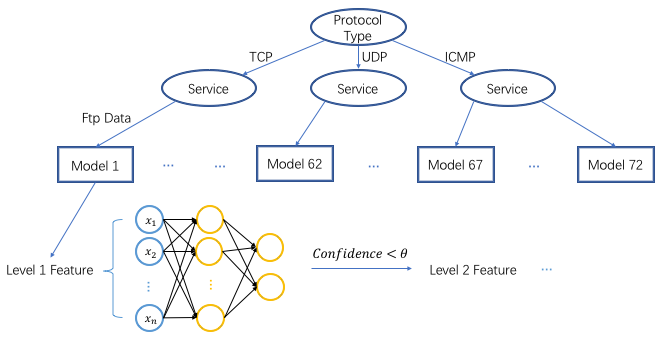
\includegraphics[scale=0.55]{img/overview}
\par\end{centering}
\caption{\label{fig:overview} An overview of the detection framework including the decision tree(top part) and the neural networks(bottom part). The total number of models are calculated on NSL-KDD dataset.}
\end{figure*}

\subsection{Cost Analysis}

\subsubsection{Computational Cost}
One of the major challenges in real-time IDSs is the computational cost attached with the system. For example, the well-known K-nearest Neighbor Classifier\cite{liao2002use} performs well on off-line datasets, but it is not an appropriate detector in real time. Because the
KNNC calculates the similarity between the new 
packet and each packet in the training set to decide the label of the new packet. So KNNC is computationally
expensive when the incoming number of packets is huge, causing the system to be overloaded.

Traditionally, less features numbers and models with less parameters will lead to low computational cost. However, this may also result in lower detection accuracy or higher false alarm rate. Different from former approaches, utilizing deep neural networks, the computing tasks can be accelerated on GPU\cite{chetlur2014cudnn}. Also, the ability to represent any non-linear function in very few hidden layers and hidden neurons make the computational expense even less.

\subsubsection{Time Cost}
It is obvious that the time delay for retrieving features simply from a network packet and extracting information from all former similar connections within a time period are quite different. Different from\cite{lee2001real}, the connection based features are utilized according to\cite{lee2001real} in this paper. The exact levels of features are presented in Tab \ref{tab:feature}.

\begin{itemize}
\item Level 1 features are basic features of individual TCP connections.
\item Level 2 features are content features within a connection suggested by domain knowledge.
\item Level 3 features are traffic features computed using a two-second time window.
\end{itemize}

\begin{table*}

\caption{\label{tab:feature}Levels of Features.}
\centering{}
\begin{tabular}{c|c|c}

\hline 
Level 1 Features & Level 2 Features & Level 3 Features\tabularnewline
\hline
Duration & Hot & Count \tabularnewline
Protocol type & Num failed logins & Serror rate \tabularnewline
Service & Logged in & Rerror rate \tabularnewline
Src bytes & Num compromised & Same srv rate \tabularnewline
Dst bytes & Root sell & Diff srv rate \tabularnewline
Flag & Su attempted & Srv count \tabularnewline
Land & Num root & Srv serror rate \tabularnewline
Wrong fragment & Num file creations & Srv rerror rate \tabularnewline
Urgent & Num shells & Srv diff host rate \tabularnewline
 & Num access files &  \tabularnewline
 & Num outbound cmds &  \tabularnewline
 & Is hot login &  \tabularnewline
 & Is guest login &  \tabularnewline
\hline

\end{tabular}
\end{table*}

Notice that the Level 3 features require iteration from the entire former two-second packet set, the time cost is extremely high compares with the lower level of features. Also, all the Level 3 features for connections coming at the same time can also be computed at the same time.

The process of utilizing different levels of features is:
\begin{itemize}
\item The lower level features are first used;
\item If the confidence of the classification is less than a threshold $\theta$, higher level features are extracted and are used combined with other lower level features;
\item If the extracted feature level is already $3$, then the eventual detection result is made without confidence calculating.
\end{itemize}
For example, both Level 1 and Level 2 features are considered after extracting the Level 2 features.

\subsection{Decision Tree Model}

Packets with different protocol types and different services tend to have different signatures to be malicious.
Thus different detectors should be trained, and for each new packet, its protocol type and service decides which detector to use. This model selection framework can be modeled by a decision tree. 

As shown in Fig \ref{fig:overview}, the decision has very simple architecture in the proposed approach.

\subsection{Neural Network Detectors}

Neural network models are at the bottom layer for the detection process, they trained for each protocol type and service respectively. Actually due to the less complexity for packets detection, neural network models perform nearly the same as traditional classifiers. The main reason of utilizing neural network models in this paper is the excellent GPU acceleration support for deep learning libraries, which will reduce the computational cost in some extent.

Neural network models with only one hidden layer is utilized in this paper, and the following experiments proves their capability for intrusion detection with such simple architectures.

\subsection{Evaluation Methods}
Three evaluation metrics are employed in this paper to evaluate the performance of the intrusion detection system, namely, detection accuracy, false alarm rate and total cost:

\begin{itemize}
\item Detection accuracy is simply calculated by comparing the predicted results with the ground truth labels.
\item The false alarm rate(FAR) is defined as Eq \ref{eq:false-alarm}, in which $FP, TN$ represent false positive and true negative samples respectively.

\begin{equation}\label{eq:false-alarm}
FAR = \frac{FP}{FP+TN}
\end{equation}

\item The total cost is the sum of the computational cost and the time cost. 
\end{itemize}

\section{Experiments}\label{sec:experiment}
\subsection{Dataset}
As mentioned in Sec \ref{sec:publicdatasets}, NSL-KDD dataset consists of the selected records of the KDD Cup 1999 dataset, which is more challenging to detect compared with the original widely used benchmark KDD Cup 1999 dataset. 
The NLS-KDD dataset solves the issues of models trained on KDD Cup 1999 dataset, which have high seemingly accuracy but actually poor capability of anomaly detection.

All the features in NSL-KDD dataset are considered in this paper except the additional feature: detection difficulty, which is generalized by statistical analysis for the KDD Cup 1999 dataset\cite{tavallaee2009detailed}. Totally, there are $61$ different TCP services, $5$ different UDP services and $6$ different ICMP services.

\subsection{Parameter Setting}
The data preprocessing method z-normalization is employed.
All the code for the neural network models is implemented in Python utilizing deep learning framework Tensorflow, and the neural network models are trained on one GPU GeForce GTX TITAN X for $5000$ epochs with early stop policy. All the neural networks consist of $1$ hidden layer, and the number of hidden neurons are set specifically for every model. The initial learning rate is $\eta = 0.0001$ and dropout ratio is $0.75$ to avoid over fitting. Finally, a softmax layer is utilized to calculate loss and Adam\cite{kingma2014adam} is employed to accelerate learning. The prediction results of the models are the values of the two output neurons.

\subsection{Baseline}
Support Vector Machine(SVM) is employed as a baseline method for each model respectively. The code are implemented in Python on Scikit-learn Library. And the following baseline results are evaluated on the same server with the proposed approach without GPU support for SVM method.

\subsection{Detection Results}
Due to the coming deadline issue, I have only finished part of the experiments.

\subsubsection{Detection Accuracy.}
Tab \ref{tab:detection-accuracy} demonstrates the detection accuracy for each level of features. And apart from the over all accuracy, I take three representative protocol type and service(TCP finger/UDP domain\_u/ICMP eco\_i) as examples.

Observed from Tab \ref{tab:detection-accuracy}, we can see that SVM models and neural network models perform nearly the same on most of the detections. But neural network models demonstrate a good property on the three examples that as the level of features get higher, the accuracies never decay; while the SVM method present less stability. Actually, this property is quite important in the proposed approach, because the accuracy decay on higher feature level will result in some eventual detection results to be wrong. Since the results for packets that cannot be classified confidently by the lower feature level models are decided finally by the higher feature level models. Also, lots of time cost will be wasted for no improvement in detection accuracy.

Also, we can observe that the decision tree idea that to detect different protocol types and service with different models is quite reasonable. In Tab \ref{tab:detection-accuracy}, huge accuracy improvement has been made thanks to this separation.

\begin{table*}

\caption{\label{tab:detection-accuracy}Detection Accuracy Results.}
\centering{}
\begin{tabular}{ccccc}

\hline 
Methods/Features & Over all & TCP finger & UDP domain\_u & ICMP eco\_i \tabularnewline
\hline
\textbf{Level 1 Features} \tabularnewline
SVM & $78.20\%$ & $99.26\%$ & $99.33\%$ & $94.27\%$ \tabularnewline
Ours & $79.16\%$ & $99.26\%$ & $99.33\%$ & $94.27\%$\tabularnewline
\hline

\textbf{Level 2 Features} \tabularnewline
 
SVM & $81.39\%$ & $97.06\%$ & $99.55\%$ & $94.27\%$\tabularnewline
Ours & $80.67\%$ & $99.26\%$ & $99.78\%$ & $94.27\%$\tabularnewline
\hline

\textbf{Level 3 Features} \tabularnewline
  
SVM & $80.57\%$ & $99.26\%$ & $99.78\%$ & $98.09\%$\tabularnewline
Ours & $76.24\%$ & $99.26\%$ & $99.78\%$ & $98.89\%$\tabularnewline
\hline
\end{tabular}
\end{table*}

\subsubsection{False Alarm Rates.}
Tab \ref{tab:detection-false-alarm} demonstrates the false alarm rates for each level of features. As mentioned before, three representative protocol type and service are presented.

As observed, the false alarm rates tends to decay as the increasing level of features. Especially, for the ICMP eco\_i models, the false alarm rates decay significantly for Level 3 features. For these type of situations, the extraction of high level features is necessary.

\begin{table*}

\caption{\label{tab:detection-false-alarm}Detection False Alarm Rates.}
\centering{}
\begin{tabular}{ccccc}

\hline 
Methods/Features & Over all & TCP finger & UDP domain\_u & ICMP eco\_i \tabularnewline
\hline
\textbf{Level 1 Features} \tabularnewline
SVM & $3.86\%$ & $0.00\%$ & $0.67\%$ & $57.69\%$ \tabularnewline
Ours & $4.40\%$ & $0.00\%$ & $0.67\%$ & $57.69\%$\tabularnewline
\hline

\textbf{Level 2 Features} \tabularnewline
 
SVM & $1.81\%$ & $0.00\%$ & $0.45\%$ & $57.69\%$\tabularnewline
Ours & $3.49\%$ & $0.00\%$ & $0.45\%$ & $57.69\%$\tabularnewline
\hline

\textbf{Level 3 Features} \tabularnewline
  
SVM & $2.19\%$ & $0.00\%$ & $0.00\%$ & $19.23\%$\tabularnewline
Ours & $6.64\%$ & $0.00\%$ & $0.00\%$ & $7.69\%$\tabularnewline
\hline
\end{tabular}
\end{table*}

\subsubsection{Cost Analysis.}
Tab \ref{tab:cost} demonstrates the \textbf{computational cost} for each level of features. The same as former experiments, three representative protocol type and service are selected. Notice here I report the average time for computing single one packet feature item. 

Thanks to GPU acceleration, it can be noticed that significant improvement have been made on computational cost utilizing neural network models, which is quite important in real time detection for the IDSs. Also the number of neurons in the hidden layer is reduced as small as possible, which also save the computational cost.

Also, \textbf{time cost} is considered. Every new packet are first detected according to their Level 1 features. If the confidence of the classification, which is the larger value of the two output neurons is less than $\theta=0.8$, than the higher features are extracted and higher level models are used. 
In the worst case, the packet will eventually get its label through Level 3 models. And more additional computational cost will also be spent. 

The total cost is the sum of computational cost and time cost. The proposed approach is much more efficient compared with simply using Level 3 features for all the packets, and there is almost no decay of detection accuracy.

\begin{table*}

\caption{\label{tab:cost}Computational Cost Results.}
\centering{}
\begin{tabular}{ccccc}

\hline 
Methods/Features & Over all & TCP finger & UDP domain\_u & ICMP eco\_i \tabularnewline
\hline
\textbf{Level 1 Features} \tabularnewline
SVM & $4.2*10^{-4}s$ & $4.4*10^{-6}s$ & $9.2*10^{-7}s$ & $5.7*10^{-7}s$ \tabularnewline
Ours & $5.4*10^{-8}s$ & $2.7*10^{-6}s$ & $4.3*10^{-7}s$ & $1.4*10^{-6}s$\tabularnewline
\hline

\textbf{Level 2 Features} \tabularnewline
 
SVM & $5.9*10^{-4}s$ & $7.3*10^{-6}s$ & $1.3*10^{-6}s$ & $1.3*10^{-6}s$\tabularnewline
Ours & $7.0*10^{-8}s$ & $2.7*10^{-6}s$ & $4.6*10^{-7}s$ & $1.4*10^{-6}s$\tabularnewline
\hline

\textbf{Level 3 Features} \tabularnewline
  
SVM & $2.3*10^{-4}s$ & $7.2*10^{-6}s$ & $4.1*10^{-6}s$ & $6.2*10^{-6}s$\tabularnewline
Ours & $1.0*10^{-7}s$ & $2.8*10^{-6}s$ & $5.2*10^{-7}s$ & $1.5*10^{-6}s$\tabularnewline
\hline
\end{tabular}
\end{table*}


\section{Future Work}\label{sec:futurework}
\subsection{More Experiments}
As mentioned in Sec \ref{sec:experiment}, due to the coming deadline, some of the experiments are not completely finished. 

The future work for this paper is listed as follows:
\begin{itemize}
\item Calculate the average performance for all the models, not for only some examples.
\item Measure the specific improvement made by distinguishing different level of features quantitatively, such as calculate the exact cost saved for detecting some packets.
\item Try more specific detection results than just normal and anomaly classification. Actually, the NSL-KDD dataset provides the labels of the specific attack types for each connection.
\end{itemize}

\subsection{More Issues}
There are also some practical issues need to be solved for further implementation:
\begin{itemize}
\item There are some protocol type and service with very few training data, such as TCP pm\_dump, UDP tftp\_u and ICMP urh\_i etc. This issue will make it impossible to train a neural network model. Maybe some signature-based technique are needed here.
\item It will cost too much time to train and tune parameters for every model, specifically $72$ models in NSL-KDD dataset. But currently I just train the example models manually.
\item Utilizing the features in NSL-KDD makes the detection in this paper to be connection based, which means that the intrusion can only be detected after all the packages in one connection have arrived. Actually, as suggested in\cite{lee2001real}, some intrusion can be detected only after the first package or a few packages are sent, which is capable to reduce the time cost even more. So extracting more package based features for model training can be considered as another improvement.
\end{itemize}

\section{Conclusion}\label{sec:conclusion}
In this paper, a new cost-based approach for fast intrusion detection is proposed. Utilizing both decision tree models and neural network models with GPU acceleration, the proposed IDS is capable of maintaining high detecting intrusion accuracy with the minimization of both computational cost and time cost. The results are evaluated on NSL-KDD dataset, and a good performance is demonstrated in the experiments.

However, as mentioned in Sec \ref{sec:futurework}, there still remains many issues to be solved for IDSs, such as how to detect intrusion only after a few packages have been received, and how to accurately detect zero-day attacks. Also, more attack simulations need to be organized to test the IDSs before they are actually employed in the real environment, since any crash in IDSs may leads to severe network problems. 

After accomplishing the rest experiments, further research will focus on solving the mentioned issues in Sec \ref{sec:futurework}. 

\bibliographystyle{ACM-Reference-Format}
\bibliography{security} 
\end{document}